\chapter{Healthcare and Life Sciences}

\section*{Why This Matters}

Healthcare and life sciences represent domains where transformer models address critical challenges with unique constraints rarely encountered in other industries. These constraints fundamentally shape architecture decisions, deployment strategies, and economic models. Clinical documentation consumes 30--40\% of physician time, yet proper documentation is essential for patient safety and billing. Medical imaging interpretation faces global specialist shortages amid increasing imaging volumes. Drug discovery timelines span 10--15 years at costs exceeding \$2 billion per approved drug. Patient risk prediction could prevent hospital readmissions affecting millions annually. Genomic analysis increasingly drives treatment selection but requires specialized interpretation.

Transformer-based systems demonstrate measurable impact: reducing documentation time by 50--70\%, achieving diagnostic accuracy comparable to specialists in specific imaging tasks, accelerating drug candidate identification by 2--5\times, and identifying high-risk patients for proactive intervention. Understanding these applications requires recognizing that healthcare AI success is determined not by model accuracy alone but by regulatory compliance, clinical adoption, patient outcomes, and organizational implementation—factors that do not apply uniformly across industries.

Regulatory requirements, accuracy thresholds where errors have clinical consequences, clinical workflow integration challenges, and liability frameworks create technical and operational constraints that fundamentally differ from consumer AI. This chapter examines healthcare and life sciences applications from an engineering perspective, focusing on technical requirements, regulatory constraints, economic considerations, and the adoption barriers that determine successful deployment in these high-stakes domains.

\section{Patient Risk Prediction and Clinical Decision Support}

\begin{figure}[htbp]
\centering
\includegraphics[width=0.95\textwidth]{chapters/diagrams/chapter12_risk_prediction_q1r2s3t4.png}
\caption{Patient risk prediction architecture showing the complete workflow from EHR data sources through model types to clinical applications and workflow integration. The system processes demographics, diagnoses, medications, lab values, and vital signs using gradient boosted trees, neural networks, or temporal models to predict readmission risk, sepsis, mortality, and high-cost patients. Implementation costs \$300K-1M with ROI of 0.2-5\times depending on scale and intervention effectiveness.}
\label{fig:risk_prediction_architecture}
\end{figure}

\subsection{Business Context and Applications}

Patient risk prediction represents the largest category of deployed healthcare AI, yet often receives less attention than more visible applications like imaging or drug discovery. These systems identify patients at elevated risk for adverse events, enabling proactive intervention before crises occur. The business case is compelling: preventing a single hospital readmission (average cost \$10,000--25,000) or detecting sepsis early (improving outcomes 10--15\%, worth \$5,000--15,000 per patient) justifies substantial investment in prediction systems.

Hospital readmission prediction targets patients likely to return within 30 days of discharge. Medicare estimates 15--20\% of discharged patients are readmitted within 30 days, costing the system approximately \$15 billion annually. Identifying even 30\% of high-risk readmissions and preventing 20\% of them through intervention saves organizations \$50,000+ annually per 1,000 discharges. The economic incentive is strong, particularly as Medicare reduces payment for readmissions exceeding quality thresholds.

Sepsis and acute deterioration detection systems monitor patients in real-time, identifying early warning signs of deterioration. Sepsis develops rapidly; early recognition and treatment dramatically improves survival. Studies show that one-hour delays in antibiotic administration for sepsis increase mortality by approximately 7\%. Early detection systems can alert clinicians to potential sepsis within 30--60 minutes, enabling faster treatment initiation. The value of preventing a single sepsis death (worth approximately \$100,000+ in outcome improvement) justifies substantial prediction system investment.

Mortality prediction systems estimate the probability of in-hospital or 30-day mortality, enabling conversations about goals of care, palliative care, and resource allocation. These systems enable physicians to identify when patients are unlikely to survive and have conversations about preferences before crisis occurs. The emotional and ethical value exceeds the economic value, but economic benefits also accrue through reduced unnecessary ICU days for patients with poor prognosis.

High-cost patient identification enables proactive care management targeting the 20\% of patients consuming 80\% of healthcare costs. Chronically ill patients benefit from care coordination, medication management, and remote monitoring. Identifying high-cost patients at the beginning of their engagement enables early intervention. Value is realized through reduced ER visits, hospitalizations, and complications through better disease management.

\subsection{Risk Prediction Architecture and Approaches}

Risk prediction systems typically use gradient boosted tree models or neural networks on structured patient data: demographics, diagnoses, procedures, medications, lab values, and vital signs. Electronic health records provide this data, though data extraction, cleaning, and integration often represent the largest implementation challenge.

Gradient boosted models (XGBoost, LightGBM, CatBoost) provide strong performance with advantages for healthcare deployment. These models are interpretable---feature importance rankings show which factors drive predictions---addressing a key healthcare requirement. They handle missing data well, which is critical for EHR data with inconsistent documentation. They are computationally efficient, enabling real-time prediction in clinical systems. The trade-off involves lower performance compared to deep learning models.

Neural network models on structured data achieve 3--8\% better performance than gradient boosted models but with reduced interpretability. Attention mechanisms can highlight which data points most influence predictions, providing some interpretability. For complex datasets with thousands of features and long history, neural networks can learn nonlinear interactions that tree models miss.

Temporal models (recurrent neural networks, temporal convolutional networks) explicitly model time series aspects of patient data: lab values changing over time, medication adjustments, symptom progression. These models naturally capture disease trajectories and deterioration patterns better than models treating all data as a single snapshot. The trade-off involves greater complexity and computational cost.

\subsection{Clinical Validation and Adoption Challenges}

Risk prediction systems require careful clinical validation. High-performing models in development often show reduced performance when deployed to new hospital systems or patient populations. This performance degradation occurs because training data may not represent deployment data: patient mix differs, documentation practices vary, hospital workflows differ, and underlying disease prevalence varies.

Prospective validation studies, where the system makes predictions on new patients before clinical outcomes are known, provide the strongest evidence. These studies demonstrate whether the system actually predicts future outcomes. Retrospective studies on historical data cannot account for changes in clinical practice, documentation, or patient mix over time.

Adopting risk prediction requires integrating with clinical workflows and EHR systems. Ideal integration places predictions in the workflow where clinicians naturally encounter information: admission summaries, shift handoffs, clinical dashboards. Predictions that require clinicians to check a separate system rarely achieve high utilization. Alert fatigue is a significant risk---clinicians may ignore systems that generate frequent alerts, even if most are accurate. Typical recommendation is that alerts should have positive predictive value exceeding 50\% for adoption; lower thresholds generate alert fatigue.

Physician acceptance depends on trust and clinical validation. Clinicians want to understand why a system made a prediction and whether they agree. Models that simply output a risk score without explanation face skepticism. Explanation methods showing which factors most influenced a prediction help clinicians evaluate prediction reasonableness.

\subsection{Economic Impact and Implementation}

The economic value of risk prediction depends on the specific application and effectiveness of interventions. For readmission prediction, preventing one readmission (cost \$10,000--25,000) through intervention generates value. If a system identifies 100 high-risk patients and 30 would have been readmitted, preventing 20\% of those through intervention saves \$60,000 (6 prevented readmissions at \$10,000 average). At \$50,000 annual system cost, ROI is marginal unless volume is higher or prevention rates are better.

For sepsis detection with one-hour earlier identification, value reaches \$5,000--15,000 per patient detected (improved survival times reduced ICU duration). Detecting 50 sepsis cases annually with 30\% improvement rate and average \$10,000 value yields \$150,000 in annual value, supporting system cost of \$30,000--50,000 monthly.

Implementation costs include EHR integration (6--12 months, \$100,000--300,000), data infrastructure (extracting, cleaning, updating patient data in real-time), model validation (clinical studies demonstrating effectiveness), and monitoring (tracking prediction accuracy over time). Total implementation cost typically reaches \$300,000--1,000,000 for health systems. This capital investment requires strong business case and executive support.

Infrastructure costs for serving prediction models at scale are modest. Scoring 10,000 patient records daily against multiple prediction models requires minimal compute: a few CPU cores suffice. The bottleneck is data extraction and integration with EHRs, not model inference.

Continuous improvement is essential for sustained success. Patient populations change, documentation practices evolve, and disease epidemiology shifts seasonally. Models that remain static degrade in performance over months. Retraining models on recent data maintains performance but requires sustained investment and governance.

\section{Clinical Natural Language Processing}

\begin{figure}[htbp]
\centering
\includegraphics[width=0.95\textwidth]{chapters/diagrams/chapter12_clinical_nlp_a1b2c3d4.png}
\caption{Clinical NLP pipeline for documentation assistance, showing the end-to-end workflow from patient-physician conversation through speech recognition, information extraction with Clinical BERT, note generation, physician review, and EHR integration. The system achieves 90-95\% accuracy and reduces documentation time by 50-70\%, providing 3-10\times ROI.}
\label{fig:clinical_nlp_pipeline}
\end{figure}

\subsection{Clinical Text Characteristics and Domain-Specific Challenges}

Clinical documentation differs fundamentally from general text in ways that affect model architecture and training strategies. Medical terminology includes highly specialized vocabulary---anatomical terms, drug names, procedure codes, disease classifications---that rarely appears in general corpora. A single clinical note might contain hundreds of domain-specific terms that general-purpose language models have never encountered during training.

Abbreviations and acronyms appear with extreme density in clinical text. ``PT'' might mean patient, physical therapy, prothrombin time, or posterior tibial, depending on context. ``MS'' could indicate multiple sclerosis, mitral stenosis, mental status, or morphine sulfate. Disambiguation requires medical knowledge and contextual understanding that general models lack. Clinical NLP systems must handle this ambiguity reliably, as misinterpretation directly affects patient care.

Temporal reasoning pervades clinical documentation. Understanding disease progression, treatment response, and medication timing requires tracking events across multiple notes spanning months or years. A phrase like ``improved since last visit'' requires identifying the previous visit, extracting relevant findings, comparing current state, and understanding the temporal relationship. This temporal reasoning exceeds the capabilities of models processing individual notes in isolation.

Negation and uncertainty require careful handling. ``No evidence of pneumonia'' means the opposite of ``evidence of pneumonia,'' yet both contain the word ``pneumonia.'' ``Possible cardiac involvement'' expresses uncertainty that affects clinical decision-making differently than ``confirmed cardiac involvement.'' Clinical NLP systems must detect and preserve these semantic distinctions, as errors directly lead to inappropriate treatment decisions.

\subsection{Clinical Language Models and Training Requirements}

Specialized clinical language models address domain-specific challenges through targeted pre-training on medical text. Clinical BERT, trained on 2 million clinical notes from MIMIC-III, achieves 3--5\% better performance than general BERT on clinical NLP tasks such as medication extraction and adverse event detection. This improvement, while seemingly modest, translates to thousands of correctly processed notes in production deployment.

BioBERT and PubMedBERT target biomedical literature rather than clinical notes, training on PubMed abstracts and full-text articles. These models excel at scientific text understanding---extracting relationships between genes, proteins, and diseases---but perform worse on clinical documentation with its abbreviations and informal language. Model selection depends on the specific application: clinical documentation assistance versus biomedical research literature analysis.

Model size for clinical applications typically ranges from 110 million to 340 million parameters (BERT-base to BERT-large). Larger models provide better performance but face deployment constraints in healthcare IT environments with limited GPU resources and conservative IT governance. Many healthcare organizations lack the infrastructure for serving multi-billion parameter models, making smaller, efficient models more practical despite lower absolute performance.

Fine-tuning clinical models requires labeled clinical data. Clinical experts---physicians, nurses, medical coders---must annotate training examples, costing \$50--200 per hour depending on specialization and task complexity. Annotating 10,000 examples for a clinical NLP task costs \$100,000--500,000. This annotation cost often exceeds model training costs, making data efficiency critical for economic viability. Organizations should carefully define annotation scope, provide detailed guidelines, and validate inter-annotator agreement before scaling annotation efforts.

\subsection{Clinical NLP Applications and Economic Value}

Clinical documentation assistance represents the highest-impact application, addressing physician burnout from documentation burden. Ambient clinical intelligence systems listen to patient-physician conversations, extract relevant information through speech-to-text and NLP, and generate clinical note drafts. These systems reduce documentation time from 2--3 hours daily to 30--60 minutes, enabling physicians to see more patients or recover working hours.

Implementation requires careful attention to accuracy and clinical workflow integration. The system must correctly capture diagnoses, medications, allergies, and treatment plans, as errors directly affect patient safety. Physicians must review and edit generated notes---notes are not simply accepted but refined. Typical accuracy targets are 90--95\% for structured information extraction (diagnoses, medications), with physician review catching remaining errors and adding nuance.

Clinical coding---assigning ICD-10 diagnosis codes and CPT procedure codes for billing---represents another application. Manual coding by certified coders costs \$2--5 per encounter. Automated coding systems achieve 70--85\% accuracy on common diagnoses and procedures, with human coders reviewing and correcting predictions. This hybrid approach reduces coding costs by 40--60\% while maintaining billing accuracy and compliance.

Clinical decision support systems extract information from clinical notes to identify patients at risk for specific conditions or complications. A system might scan notes to identify patients with uncontrolled diabetes, overdue cancer screenings, or drug interaction risks. These systems must achieve high recall (finding all relevant cases) while maintaining acceptable precision (avoiding false alarms). Typical targets are 85--95\% recall and 70--85\% precision.

Economic analysis for clinical documentation assistance is compelling. A physician earning \$200,000--400,000 annually spending 30--40\% of time on documentation represents \$60,000--160,000 annual cost. Reducing documentation time by 60\% saves \$36,000--96,000 per physician. At \$10,000--30,000 annual system cost per physician, ROI is 2--10\times. Implementation across 100 physicians saves \$3.6--9.6 million annually, supporting substantial investment.

\section{Medical Imaging and Computer Vision}

\begin{figure}[htbp]
\centering
\includegraphics[width=0.95\textwidth]{chapters/diagrams/chapter12_medical_imaging_e5f6g7h8.png}
\caption{Multimodal medical imaging architecture combining vision transformers for image processing with Clinical BERT for text encoding. Cross-attention mechanisms enable fusion of visual and clinical context, achieving 5-10\% better accuracy than image-only models. The system requires 8-16 GB GPU memory for inference and must undergo FDA validation.}
\label{fig:medical_imaging_architecture}
\end{figure}

\subsection{Vision Transformers for Medical Imaging}

Medical imaging applications---radiology, pathology, dermatology, ophthalmology---face global specialist shortages and increasing imaging volumes. Vision transformers applied to medical images achieve diagnostic accuracy comparable to specialists for specific, well-defined tasks: detecting pneumonia on chest X-rays (95\%+ accuracy), identifying diabetic retinopathy in fundus photographs (90\%+ accuracy), or classifying skin lesions.

Medical images differ from natural images in ways that affect model architecture. Images are often high-resolution (2000\times2000 pixels or larger for CT/MRI), grayscale or specialized color spaces (for different imaging modalities), and contain subtle features critical for diagnosis. A 2mm lung nodule in chest CT might be the only sign of early cancer, requiring models to detect tiny features in large images.

Vision transformer architectures for medical imaging use patch sizes of 16\times16 or 32\times32 pixels, dividing a 2000\times2000 image into 3,900--15,600 patches. Processing this many patches requires substantial memory and computation. A ViT-Large model processing a 2000\times2000 image requires approximately 24 GB of memory during training, necessitating high-end GPUs or gradient checkpointing techniques. Alternative architectures (Swin transformers, hierarchical approaches) reduce computational requirements by processing images at multiple resolutions.

Transfer learning from natural images (ImageNet pre-training) provides limited benefit for medical imaging. ImageNet pre-training helps with general visual features (edges, textures) but doesn't capture medical-specific patterns (lung infiltrates, cellular morphology, tissue density variations). Domain-specific pre-training on medical image datasets (ChestX-ray14, MIMIC-CXR) provides better performance. These medical datasets are smaller than ImageNet, limiting pre-training benefits, but the domain-specific knowledge justifies pre-training.

\subsection{Modality-Specific Considerations}

Radiology applications (X-ray, CT, MRI, ultrasound) have different characteristics affecting model architecture and deployment. X-ray is two-dimensional, high-volume (100+ per radiologist daily), and relatively fast to interpret. AI systems can process X-rays quickly, enabling throughput increases. CT and MRI are three-dimensional, requiring models to process volumetric data (10\times more data than 2D). Processing 3D data requires either volumetric neural networks (computationally expensive) or 2D slice-by-slice approaches (missing 3D context).

Pathology deals with gigapixel images (40,000\times40,000 pixels or larger) from slide scanners. Standard image processing approaches fail because the entire image doesn't fit in GPU memory. Specialized approaches divide images into tiles, process tiles independently, then aggregate results. These approaches must handle tile boundaries carefully to avoid missing structures spanning multiple tiles.

Dermatology faces different challenges. Standardized photography is critical---lighting, angle, and distance affect appearance. Variability in photography makes models less reliable. However, clinical stakes are typically lower (skin conditions are rarely life-threatening), and treatment decisions are often clear. Dermatology AI adoption is relatively high because risk is low and benefit is clear.

Ophthalmology involves specialized imaging equipment (fundus cameras, optical coherence tomography) producing images optimized for specific diseases. Models trained on fundus images for diabetic retinopathy may not generalize to other retinal diseases. Modality-specific training data is essential.

\subsection{Multimodal Clinical Models}

Combining medical images with clinical text enables richer understanding than either modality alone. A chest X-ray interpreted with the patient's clinical history, symptoms, and prior imaging provides more accurate diagnosis than the image alone. Multimodal models that process both images and text achieve 5--10\% better diagnostic accuracy than image-only models.

Architecture for multimodal models typically uses separate encoders for each modality---a vision transformer for images, a language model for text---with cross-attention mechanisms enabling interaction. The text encoder processes clinical history, prior reports, and symptom descriptions. The vision encoder processes the current image. Cross-attention allows the model to focus on image regions relevant to mentioned symptoms or findings.

Training multimodal models requires paired image-text data. Radiology reports paired with images provide natural training data, but report quality varies. Some reports are detailed and specific; others are brief and generic. Data curation to identify high-quality image-report pairs improves model performance but requires clinical expertise.

Computational requirements exceed single-modality models. Processing a 2000\times2000 image with a 500-token clinical history requires approximately 32 GB of memory during training. Inference requires 8--16 GB. These resource requirements necessitate GPU deployment for real-time clinical use.

\subsection{Clinical Deployment and Regulatory Requirements}

Medical imaging AI systems require FDA approval as medical devices under the Software as Medical Device (SaMD) framework. This regulatory requirement involves demonstrating safety and effectiveness through clinical studies with hundreds to thousands of cases. Validation costs \$500,000--2,000,000 and takes 12--24 months, substantially increasing time-to-market and development costs.

Clinical validation requires demonstrating performance on diverse patient populations, imaging equipment, and clinical settings. A model trained on academic medical center data might perform poorly on images from community hospitals with different equipment or patient demographics. Validation datasets must represent the intended use population, requiring multi-site data collection and careful attention to demographic diversity.

Continuous monitoring after deployment detects performance degradation. Imaging equipment changes, patient populations shift, and disease epidemiology varies over time. These changes degrade model performance, requiring retraining or recalibration. Monitoring systems track prediction confidence, error rates, and distribution shift, alerting when performance falls below acceptable thresholds.

Liability and responsibility frameworks affect deployment. If an AI system misses a diagnosis, who is liable---the physician, healthcare organization, or AI vendor? Current practice treats AI as decision support, with physicians retaining ultimate responsibility. This framework requires physicians to review and validate AI predictions, limiting automation potential. As confidence in AI systems increases, liability frameworks will evolve, potentially enabling greater automation with appropriate safeguards.

\section{Genomics and Precision Medicine}

\subsection{Genetic and Genomic AI Applications}

Genomic analysis increasingly drives clinical decisions: identifying pathogenic genetic variants, determining cancer mutation profiles that guide treatment selection, and assessing pharmacogenomic variants that affect drug metabolism. Transformer models and other machine learning approaches are being applied to genetic data with increasing clinical impact.

Variant interpretation---determining whether a genetic variant is pathogenic, benign, or uncertain---is a critical bottleneck. Clinically actionable genetic testing produces thousands of variants per patient, most of which are benign. Computational tools must prioritize which variants deserve expert review. Machine learning models trained on databases of known pathogenic variants (ClinVar, HGMD) predict pathogenicity of novel variants. Performance reaches 85--92\% accuracy on well-studied genes.

Cancer genomics has transformed clinical oncology. Tumor sequencing identifies mutations in cancer-causing genes, determining which treatments are likely effective. For example, mutations in EGFR in lung cancer predict response to specific targeted therapies; mutations in BRCA1/2 affect breast cancer treatment strategy. Machine learning predicts treatment response from mutation profiles with 75--85\% accuracy.

Pharmacogenomics analyzes genetic variants affecting drug metabolism. Variations in cytochrome P450 enzymes determine whether patients metabolize certain drugs quickly (requiring higher doses) or slowly (risking toxicity). Genetic testing predicts optimal dosing for many medications. The economic value is high: preventing adverse drug events costs \$5,000--20,000 per event avoided.

Rare disease diagnosis uses genetic variants to match patients to disease causes. Rare genetic diseases often have multiple possible causes; genetic sequencing identifies mutations and machine learning determines most likely diagnosis. This genetic diagnosis enables appropriate treatment and prognosis counseling.

\subsection{Technical Approaches and Validation}

Machine learning approaches for genomic analysis range from sequence-based (processing DNA sequences directly) to variant-based (processing individual genetic variants) to multi-omics (combining genomic, transcriptomic, proteomic data).

Sequence-based approaches use language models trained on DNA sequences. DNA can be represented as text (A, T, G, C nucleotides), enabling direct application of NLP methods. Nucleotide transformers trained on billions of base pairs learn sequence patterns associated with function and disease. These models predict mutation effects, pathogenic variants, and regulatory changes from sequence alone.

Variant-based approaches treat individual genetic variants as features. A patient is represented as a vector of presence/absence of specific variants. Gradient boosted models or neural networks predict phenotypes (disease presence, treatment response) from variant profiles. These approaches are computationally simpler than sequence-based approaches but don't leverage the information in variant context.

Multi-omics approaches combine genomic, transcriptomic (which genes are expressed), proteomic (protein abundance), and metabolomic (chemical byproducts) data. Integration of these data types provides richer understanding of disease biology. Transformer-based multi-omics models achieve better disease prediction than single-omics approaches.

Regulatory requirements for genomic AI are evolving. CLIA (Clinical Laboratory Improvement Amendments) governs clinical genetic testing. FDA oversight of genomic AI is increasing for high-stakes applications (cancer diagnosis, pharmacogenomics). HIPAA requirements apply as genetic data is part of medical records. Regulatory landscape is complex and changing, requiring careful monitoring.

\subsection{Economic Impact and Adoption}

Economic value of genomic AI depends on the specific application. Variant interpretation reduces time spent on manual curation: experts reviewing variants manually cost \$100--500 per variant. Automated interpretation with 85\%+ accuracy reduces expert time by 80\%, saving \$80--400 per variant. For a diagnostic lab processing 10,000 variants annually, savings reach \$800,000--4,000,000.

Cancer genomics AI guiding treatment selection enables better outcomes and cost optimization. Patients receiving treatment matched to their tumor profile see better response rates and fewer adverse effects. Value per correct prediction: \$20,000--100,000 (improved survival, reduced unnecessary treatment).

Pharmacogenomics testing prevents adverse drug events with value of \$5,000--20,000 per event prevented. For a population on multiple medications, genetic testing could prevent 5--10 adverse events per 1,000 patients annually. At \$100 per test, costs are offset within a year.

\section{Drug Discovery and Molecular Design}

\begin{figure}[htbp]
\centering
\includegraphics[width=0.95\textwidth]{chapters/diagrams/chapter12_drug_discovery_i9j0k1l2.png}
\caption{AI-driven drug discovery workflow showing the complete pipeline from target identification through molecular generation, virtual screening, experimental validation, and lead optimization. The iterative process reduces discovery timelines from 3-5 years to 1-2 years, providing \$200-400M savings per successful drug with 10-80\times ROI for successful programs.}
\label{fig:drug_discovery_workflow}
\end{figure}

\subsection{Molecular Representation and Property Prediction}

Drug discovery applications use transformers to model molecular structures and predict properties. Molecules can be represented as SMILES strings (text notation), molecular graphs, or 3D conformations. Each representation has different characteristics affecting model architecture.

SMILES (Simplified Molecular Input Line Entry System) represents molecules as text strings, enabling direct application of language models. The SMILES string ``CC(=O)OC1=CC=CC=C1C(=O)O'' represents aspirin. Language models trained on SMILES strings learn chemical grammar and generate novel molecules. However, SMILES has limitations: multiple SMILES strings can represent the same molecule, and small string changes can produce very different molecules.

Graph neural networks treat molecules as graphs with atoms as nodes and bonds as edges. Graph transformers apply attention to molecular graphs, learning relationships between atoms. This representation naturally captures molecular structure.

Property prediction estimates a molecule's solubility, toxicity, binding affinity, or metabolic stability. Models trained on molecular property databases achieve correlation coefficients of 0.7--0.9 with experimental measurements for well-studied properties. This accuracy enables virtual screening of millions of candidates, identifying promising molecules for experimental testing.

\subsection{Generative Models for Drug Design}

Generative models create novel molecular structures with desired properties, accelerating lead compound identification. These models learn the distribution of drug-like molecules from databases of known drugs and bioactive compounds, then generate new molecules from this learned distribution.

Conditional generation targets specific properties. A model might generate molecules with high binding affinity to a target protein, low toxicity, and favorable pharmacokinetics. Multi-objective optimization is challenging, as properties often trade off: molecules with high binding affinity might have poor solubility.

Validation requires experimental testing. Synthesizing and testing a single compound costs \$5,000--50,000 and takes weeks to months. Generative models must achieve high hit rates---the fraction of generated molecules showing desired activity---to justify experimental costs. Current models achieve 5--20\% hit rates for well-defined targets, versus 0.1--1\% random screening.

Integration with experimental workflows determines practical impact. Generative models producing molecules difficult or impossible to synthesize provide limited value. Synthetic accessibility constraints during generation---favoring molecules synthesizable with available chemistry---improves utility. This requires combining learned models with rule-based chemical knowledge.

\subsection{Protein Structure and Design Applications}

Protein language models, trained on millions of protein sequences, learn relationships between sequence and structure. ESM-2, trained on 250 million protein sequences, achieves state-of-the-art protein structure prediction and function annotation from sequence alone.

Protein structure prediction, exemplified by AlphaFold2's revolutionary results, uses transformer-based architectures to predict 3D structure from amino acid sequence. While AlphaFold2 uses specialized architectures beyond standard transformers, the attention mechanism is central. Accurate structure prediction enables drug discovery by identifying binding sites and predicting drug-protein interactions computationally.

Antibody design applies transformers to generate antibody sequences with desired binding properties. Antibodies are proteins with variable regions determining binding specificity. Generative models trained on antibody sequence databases design novel antibodies targeting specific antigens, accelerating therapeutic antibody development.

\subsection{Impact on Drug Discovery Timelines and Economics}

Drug discovery traditionally spans 10--15 years and costs exceeding \$2 billion per approved drug. This timeline breaks down roughly as: 3--6 years target identification and lead optimization (preclinical), 6--7 years clinical trials (Phase I, II, III), and 1--2 years FDA review. AI can dramatically accelerate preclinical stage, potentially reducing it from 3--6 years to 1--2 years. Clinical trials, which represent the majority of cost and timeline, are much harder to accelerate.

Preclinical time savings directly reduce time-to-first-human-trial, accelerating revenue generation for successful drugs. A two-year reduction in preclinical time, with appropriate discounting for time value of money and success rate changes, can be worth \$200--400 million per successful drug through reduced pre-revenue costs and earlier revenue start.

Hit rate improvements (finding more promising candidates earlier) reduce experimental costs and increase probability of advancing to clinical trials. If AI enables 20\% improvement in early-stage hit rates, this reduces the number of compounds requiring expensive synthesis and testing.

However, clinical trials remain expensive and time-consuming regardless of AI progress. Phase III trials for major indications cost \$400--1000 million and take 2--4 years, depending on indication and required patient population. AI can improve trial design (patient selection, endpoint selection) but cannot eliminate the fundamental requirement for human data.

\section{Implementation and Governance}

\subsection{Healthcare IT Integration and Deployment}

Healthcare AI systems must integrate with complex IT infrastructure: electronic health records, picture archiving systems, laboratory systems, pharmacy systems, and clinical workflows. Integration complexity often exceeds model development complexity, consuming 60--80\% of deployment effort.

EHR integration requires handling diverse data formats, inconsistent data quality, and vendor-specific APIs. Epic, Cerner, and other vendors provide different integration mechanisms with varying capabilities. HL7 FHIR standards improve interoperability but adoption remains incomplete. Integration projects require 6--12 months of engineering effort.

Real-time requirements for clinical decision support create latency constraints. Systems alerting physicians to drug interactions must respond within seconds to avoid disrupting workflow. Batch processing overnight suffices for population analytics but not for point-of-care support.

Data privacy and security exceed typical enterprise standards. HIPAA mandates encryption, access controls, audit logging, and breach procedures. Cloud deployment requires Business Associate Agreements with providers. These requirements add complexity and cost.

\subsection{Clinical Validation and Regulatory Approval}

Clinical validation requires demonstrating that AI systems improve patient outcomes. A model with 95\% accuracy might not improve outcomes if physicians don't trust or act on predictions.

Randomized controlled trials provide strongest evidence but are expensive and time-consuming: \$1--5 million, 12--24 months. Observational studies are faster and cheaper but weaker: \$100,000--500,000, 6--12 months.

Publication in peer-reviewed journals establishes credibility before clinical adoption. The publication process adds 6--12 months to evidence generation timelines.

Reimbursement codes and payer negotiations determine financial viability. Without reimbursement, healthcare organizations lack financial incentive to adopt.

\subsection{Fairness, Bias, and Equity}

Healthcare AI models often exhibit bias across demographic groups. Models trained predominantly on one demographic perform worse on others. Historical bias in training data encodes past discrimination. This affects equitable access to AI benefits.

Fairness metrics and mitigation strategies are critical. Sensitivity and specificity may differ across demographic groups; equity requires understanding and addressing these differences.

FDA guidance increasingly requires algorithmic fairness assessment. Demonstrating equitable performance across demographic groups becomes part of regulatory approval.

Monitoring after deployment should track performance across demographic groups, alerting when disparities emerge. This requires collecting demographic data and analyzing performance stratified by demographics.

\subsection{Operational Monitoring and Continuous Improvement}

Deployed systems degrade over time as patient populations change, disease epidemiology shifts, and clinical practices evolve. Continuous monitoring detects performance degradation and triggers retraining.

Monitoring infrastructure tracks prediction accuracy, confidence distributions, and error patterns. Alerts trigger when performance falls below thresholds.

Model monitoring costs approximate 10--20\% of initial development cost annually, making it essential to budget for sustained operations, not just initial deployment.

Continuous improvement processes collect feedback from clinical users, identify failure modes, and improve models. This organizational capability determines long-term success more than initial model quality.

\section{Economic Analysis and Return on Investment}

\begin{figure}[htbp]
\centering
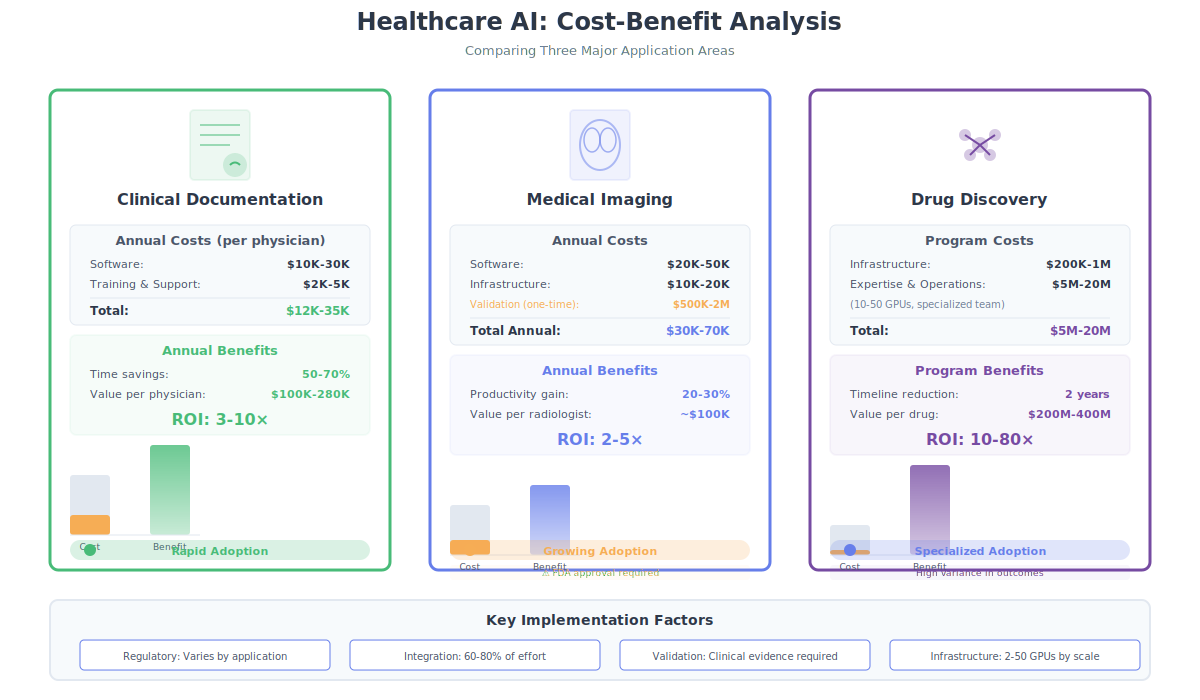
\includegraphics[width=0.95\textwidth]{chapters/diagrams/chapter12_cost_benefit_m3n4o5p6.png}
\caption{Cost-benefit analysis comparing three major healthcare AI applications. Clinical documentation provides the highest adoption rate with 3-10\times ROI at \$12K-35K annual cost per physician. Medical imaging requires FDA approval and provides 2-5\times ROI. Drug discovery demands \$5M-20M investment but offers 10-80\times ROI for successful programs with high outcome variance.}
\label{fig:healthcare_cost_benefit}
\end{figure}

Healthcare AI economics are application-specific, with wide variation in ROI and implementation complexity.

\textbf{Patient risk prediction}: \$50,000--500,000 annual value per health system (depending on scale and intervention effectiveness) at \$100,000--300,000 implementation cost. ROI is 0.2--5\times depending on scale and success of interventions. Implementation complexity is medium. Value is sustained with proper monitoring and continuous improvement.

\textbf{Clinical documentation}: \$3.6--9.6 million annual value for 100 physicians (per physician savings) at \$1--3 million implementation cost. ROI is 2--10\times. Implementation complexity is high due to workflow integration. Value is immediate upon deployment with rapid adoption.

\textbf{Medical imaging}: \$100,000 annual value per radiologist (25\% productivity improvement) at \$50,000--100,000 implementation cost. ROI is 1--2\times per radiologist, with compounding benefits across radiology departments. Implementation complexity is medium. FDA approval adds 12--24 months and \$500,000--2,000,000 cost but is mandatory for clinical deployment.

\textbf{Drug discovery}: \$200--400 million value per successful drug (through timeline compression and success rate improvement) at \$5--20 million investment in AI platform and expertise. ROI is 10--80\times for successful programs, but outcome variance is high---unsuccessful programs yield minimal return. Implementation complexity is high; scientific expertise required.

\textbf{Genomic analysis}: \$500,000--4,000,000 annual value in reduced interpretation costs at \$100,000--500,000 implementation cost. ROI is 1--40\times depending on application and volume. Implementation complexity is medium.

Infrastructure costs vary by application. Clinical NLP and risk prediction require modest compute (standard servers with GPUs). Medical imaging requires 4--8 GPUs for enterprise deployment. Drug discovery platforms require 10--50 GPUs. Monthly cloud costs range from \$1,000 to \$25,000 depending on application.

\section{Key Insights}

\textbf{Patient Risk Prediction is the Largest Deployed Category}: While imaging and drug discovery attract attention, risk stratification systems are deployed at scale across healthcare organizations. Identifying high-risk patients enables proactive intervention, preventing readmissions and adverse events. This category deserves equivalent emphasis to more visible applications.

\textbf{Domain Specialization is Essential}: General-purpose models perform poorly on clinical text due to specialized terminology, dense abbreviations, and medical reasoning. Clinical BERT and biomedical models achieve 3--5\% better performance than general models, translating to thousands of correctly processed notes in production.

\textbf{Integration and Workflow Complexity Determine Success}: Technical model quality is necessary but insufficient. Integration with EHRs, PACS, clinical workflows, and identity systems consumes 60--80\% of effort. Deployment success depends more on integration execution than on model performance.

\textbf{Regulatory Requirements Dominate Timelines}: FDA approval for medical devices requires 12--24 months and costs \$500,000--2,000,000. Clinical validation and evidence generation consume 60--80\% of total development effort. Organizations should budget appropriately for regulatory pathways.

\textbf{Accuracy Thresholds are Non-Negotiable}: Healthcare applications require 90--95\% accuracy for clinical use, as errors directly affect patient safety. This accuracy requirement necessitates extensive validation, human review workflows, and continuous monitoring.

\textbf{Economic Value Varies Dramatically by Application}: Clinical documentation provides 2--10\times ROI through physician time savings. Medical imaging provides 1--2\times ROI per radiologist. Drug discovery provides 10--80\times ROI for successful programs with high outcome variance. Risk prediction provides 0.2--5\times ROI depending on scale and intervention success. Organizations should evaluate each application on its specific economics.

\textbf{Physician Adoption is the Largest Barrier}: Even highly accurate systems fail to deliver value if physicians don't trust or use them. Building trust requires clinical validation, transparency in model decision-making, and seamless workflow integration. Adoption timelines extend 6--12 months beyond technical deployment.

\textbf{Fairness and Equity Matter for Both Ethics and Regulation}: Healthcare AI systems often exhibit performance disparities across demographic groups. Regulatory bodies increasingly require fairness assessment. Organizations should monitor performance across groups and implement bias mitigation strategies.

\textbf{Continuous Monitoring and Improvement are Essential}: Deployed systems degrade over time. Continuous monitoring, periodic retraining, and adaptation to changing clinical conditions sustain value. Budget for ongoing operations approximating 10--20\% of initial development cost annually.

The next chapter examines legal and compliance applications, where transformer models address document review, contract analysis, and regulatory compliance with unique accuracy and explainability requirements fundamentally different from healthcare's clinical validation paradigm.

